\myChapter{Datasource- und Domain Layer}\label{chap:datasourcelayer}
In diesem Kapitel sollen der Datasource- und Domain Layer der Gesamtarchitektur
vorgestellt werden. Bei der Definition des Datasource Layer wird dabei kurz auf
die Systeme eingegangen, mit denen eine Anwendung üblicherweise kommuniziert.
Anschließend werden die drei Kompenenten des Domain Layer und deren Aufgaben
näher diskutiert.

\section{Datasource Layer}\label{sec:datasource}
Der Datasource Layer stellt die unterste Schicht einer Anwendung dar und dient
dazu, eine Verbindung mit anderen Systemen herzustellen, die Aufgaben
übernehmen, die nicht von der Anwendung selbst ausgeführt werden (vgl.
\cite{fowler:2002} S. 20). In den meisten Fällen handelt es sich bei diesen Systemen um eine oder
mehrere Datenbanken, die zur permanenten Speicherung von Daten dienen. Aber auch
andere, für die Weiterverarbeitung der Daten zuständige Anwendungen können
angesprochen werden. Die für die Verbindung notwendigen Bibliotheken sollen im
folgenden allgemein als \emph{Connector} bezeichnet werden. Mögliche entfernte
Systeme für die Kommunikation sind:

\begin{description}
\item[Relationale Datenbanken] Die meisten Anwendungen kommunizieren primär mit
einem \ac{RDBMS}, das die dauerhafte Speicherung der Daten in einer relationalen
Tabellenstruktur übernimmt. Der Datasource Layer stellt hierfür eine
programmiersprachenspezifische Schnittstellentechnologie zur
Verfügung\footnote{In Java wird hierfür JDBC verwendet}, über die mit der
Abfragesprache \ac{SQL} mit einem oder mehreren \ac{RDBMS} kommuniziert werden
kann. Die Vorteile von \ac{RDBMS} sind eine solide und zuverlässige technische
Grundlage sowie die Tatsache, dass ein Großteil der Entwickler bereits mit
\ac{SQL} vertraut ist.
\item[NoSQL Datenbanken] Treten aber gleichzeitig ein hohes Anfragevolumen und
sehr große Datenmengen auf, kann die Skalierbarkeit von \ac{RDBMS} an ihre
Grenzen stoßen. Auch kann es sein, dass eine relationale Tabellenstruktur nicht
immer die optimale Lösung für die Speicherung von Daten darstellt. Für diese
Zwecke wurden Datenbanklösungen entwickelt, die Anfang 2009 erstmals allgemein
unter dem Begriff der NoSQL Datenbanken zusammengefasst wurden (siehe
\cite{wiki:nosql}). Um eine bessere Skalierbarkeit und Flexibilität zu
erreichen, wird bei vielen dieser Datenbanken auf eine feste Schemadefinition verzichtet.
Auch eine Abfragesprache wie \ac{SQL} ist meist nicht vorhanden. Um Abfragen
durchzuführen gibt es die Möglichkeit des \emph{Query-by-example}. Dabei wird ein
Beispielobjekt an die Datenbank übergeben, die alle dazu passenden Objekte
zurückliefert. Auch bieten manche Datenbanken die Möglichkeit Suchalgorithmen in
einer Programmiersprache zu implementieren, die nativ auf der Datenbank
ausgeführt werden können. In einfachen Ausprägungen können NoSQL Datenbanken
auch lediglich ein verteiltes assoziatives Array zur Verfügung stellen, in denen
gespeicherte Elemente durch einen bekannten eindeutigen Bezeichner referenziert
werden. Tabelle \ref{tab:nosql} zeigt eine Auswahl einiger NoSQL Datenbanken, die
vor allem in großen Webanwendungen häufiger zum Einsatz kommen.
\item[Entfernte Anwendungen] Entfernte Anwendungen (\emph{Remote
Application}) übernehmen Aufgaben, die nicht in der Anwendung selbst
implementiert wurden. So kann beispielsweise ein Online Shop mit einem
Warenwirtschaftssystem kommunizieren, das Bestellungen bearbeitet und verbucht.
Die Kommunikation mit anderen entfernten Anwendungen erfolgt üblicherweise über
ein \ac{RPC} Protokoll. Dabei stellt der Datasource Layer eine Klassenbibliothek
für das entsprechende Protokoll zur Verfügung, die dann von übergeordneten Schichten
verwendet wird.
\end{description}

\begin{table}[h]
	\begin{tabularx}{\textwidth}{lXX} \toprule
    	\tableheadline{Name} &
    	\tableheadline{URL} & 
    	\tableheadline{Bemerkung} \\
    	\midrule
    	Db4O & \url{http://www.db4o.com} & Objektorientiert für Java
    	und .NET \\ 
    	CouchDb & \url{http://couchdb.apache.org} &
    	Dokumentorientiert \\
    	Neo4J & \url{http://neo4j.org} & Speichert Objektgraphen \\
    	Memcachedb & \url{http://memcachedb.org/} & Verwendet Memcached Protokoll
    	\\
    	Cassandra & \url{http://incubator.apache.org/cassandra/} & Tabellenorientiert \\
		\bottomrule
	\end{tabularx}
	\captionof{table}[Auswahl einiger NoSQL Datenbanken]{Auswahl einiger NoSQL
	Datenbanken\footnotemark}
	\label{tab:nosql}
\end{table}
\footnotetext{Quelle: \cite{wiki:nosql}}

Abbildung \ref{ill:datasource} zeigt die Einordnung des Datasource Layer in die in
Kapitel \ref{chap:introduction} vorgestellte Gesamtarchitektur.

\begin{figure}[bth]
    \center{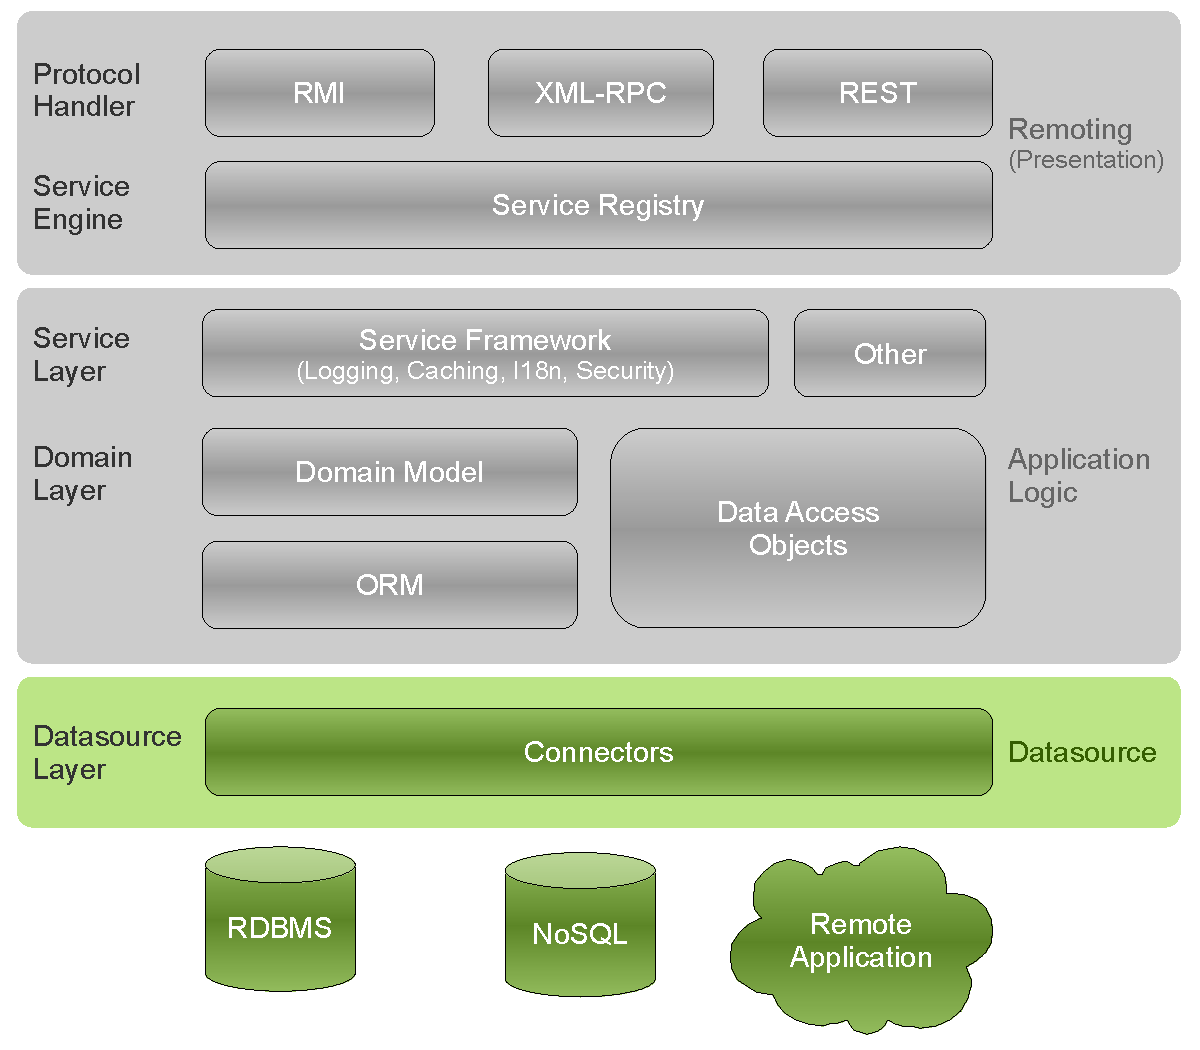
\includegraphics[width=\linewidth]{images/overviews/datasource}}
	\caption{Einordnung des Datasource Layer}
	\label{ill:datasource}
\end{figure}

\pagebreak
\section{Domain Layer}
Die dem Datasource Layer übergeordnete Schicht ist der Domain Layer. Er
beinhaltet einen Großteil der Anwendungslogik und die dafür notwendige
Kommunikation mit dem Datasource Layer. Daran sind verschiedene Komponenten
beteiligt, die nachfolgend vorgestellt werden sollen.

\subsection{Domain Model}\label{sec:domainmodel}
Das Domain Model ist die Beschreibung aller in einer Anwendung verwendeten Daten,
deren Abhängigkkeiten voneinander und den Operationen, die darauf ausgeführt
werden (siehe \cite{stoyanova:2006}). Der Entwurf des Domain Model ermöglicht
eine konzeptionelle Sicht auf das Gesamtsystem und hilft dabei, das Verständnis
für die gewünschten Funktionalitäten und das Datenmodell der Anwendung herzustellen und
zu verifizieren. In modernen Programmiersprachen stellt das Domain Model dann
eine objektorientierte Abbildung dieses Datenmodells dar. Umgesetzt wird die
Beschreibung des Domain Models oft als \ac{UML} Klassendiagram, woraus sich dann
problemlos die Klassenstruktur in einer beliebigen objektorientierten
Programmiersprache erstellen lässt. Analog zu der Terminologie der
objektorientierten Programmierung soll im weiteren Verlauf die Definition einer
einzelnen Klasse des Domain Models als \emph{Domain Klasse} und eine Instanz
dieser Klasse als \emph{Domain Objekt} bezeichnet werden.

Für die Implementierung der Anwendungslogik gibt es zwei unterschiedliche Ansätze
(vgl. \cite{fowler:2002} S. 116 - 124). Zum einen ist es möglich, diese direkt
in den Domain Klassen zu implementieren. Das hat den Vorteil, das alle Daten und
Operationen an einer Stelle gekapselt werden und direkt ersichtlich sind. Ein
Nachteil ergibt sich daraus dann, wenn die Domain Klassen sehr viel
Anwendungslogik enthalten und dadurch sehr unübersichtlich werden können. Hinzu
kommt, dass eine Domain Klasse dadurch nur schwer in anderen Anwendungen oder anderen Teilen
der Anwendung wiederverwendet werden kann. Oft ist es auch nicht möglich, auf
diese Art Operationen zu implementieren, die auf verschiedenen Domain Klassen
arbeiten. Die andere Möglichkeit besteht darin, Domain Klassen teilweise oder
vollständig als reine Datencontainer zu benutzen und die Anwendungslogik in den
in Kapitel \ref{chap:servicelayer} näher vorgestellten Service Layer auszulagern.
Auch wenn die notwendige Vereinfachung die tatsächlichen Vorteile eines Domain
Model nicht optimal veranschaulicht, soll Abbildung \ref{ill:domainmodel} die
Idee des Domain Model näher illustrieren.

\begin{figure}[bth]
    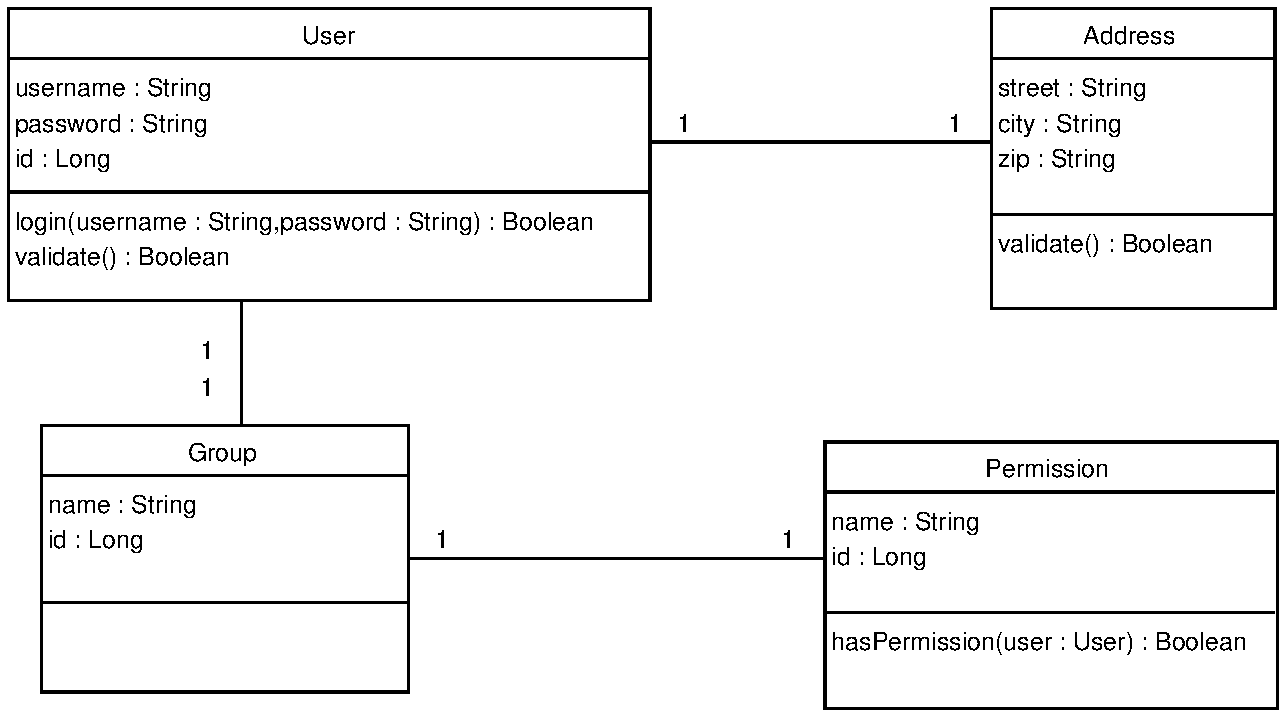
\includegraphics[width=\linewidth]{images/uml/domainmodel}
	\caption{Beispiel eines einfachen Domain Model UML Diagramms}
	\label{ill:domainmodel}
\end{figure}

Für beide Implementierungsansätze ist es aber weiterhin sinnvoll,
Funktionalitäten, die die Konsistenz des Domain Models sicherstellen, den Domain
Klassen selbst zu überlassen. Darunter fällt etwa die Prüfung auf die Einhaltung
bestimmter Geschäftsregeln, deren Nichtbeachtung einen unzulässigen Zustand des
gesamten Domain Models zur Folge hätte \footnote{Einfache Beispiele sind die
Validierung einer E-Mail Adresse oder sicherzustellen, dass ein Benutzername nur
einmal vorkommt}. Da diese Art der Validierung meist sehr stark von den Daten der
Domain Objekte abhängig ist, sollte sie ebenfalls an dieser Stelle implementiert
werden.

\subsection{Data Access Objects}
Auch wenn das Domain Model die Anwendungslogik enthält, ist es oft sinnvoll, die
Domain Objekte von der Verbindung zum Datasource Layer zu entkoppeln. Das
bedeutet dann, dass der Datasource Layer verändert werden kann, beispielsweise
durch einen Wechsel von einem \ac{RDBMS} zu einer NoSQL Datenbank, ohne das die
Domain Objekte angepasst werden müssen. Für diesen Zweck werden \emph{Data Access
Objects} (für die Java Spezifikation siehe \cite{sun:dao}) verwendet, die auf den
Domain Objekten arbeiten und mit dem Datasource Layer kommunizieren. Meist
existiert eine \ac{DAO} Implementierung für jeweils eine Domain Klasse. Ein
\ac{DAO} kann als Vermittler zwischen dem Datasource Layer, dem Domain Model und
dem Benutzer, also der Schicht über dem Domain Layer, gesehen werden. Dieser
Benutzer arbeitet weiterhin mit Domain Objekten, hat aber zusätzlich in den
verschiedenen \ac{DAO} Klassen Methoden zur Verfügung, die Domain Objekte aus dem
Datasource Layer lesen. Die Implementierung eines \ac{DAO} übernimmt in diesen
Methoden dann die Kommunikation mit dem Datasource Layer und die Erstellung
passender Domain Objekte.

\subsection{Object-Relational Mapping}\label{subsec:orm}
Die häufigste Aufgabe eines \ac{DAO} ist die Instanziierung von Domain Objekten
aus den Ergebnissen von \ac{SQL} Abfragen auf einer relationalen Datenbank. Die
objektorientierte Darstellung des Domain Model lässt sich nämlich nur sehr selten
direkt in eine relationalen Tabellenstruktur übertragen. Für die Konvertierung
der Darstellungen gibt es verschiedene Lösungsmöglichkeiten. Die verschiedenen
Ansätze werden in \cite{fowler:2002} Kapitel 10 - 14 näher behandelt. Hier soll
der verwendete Ansatz der Object-Relational Mapping Frameworks näher behandelt
werden.

Grundsätzlich müssen die Ergebnisse einer \ac{SQL} Abfrage an das \ac{RDBMS} auf
die entsprechenden Domain Objekte übertragen werden, was sich am einfachsten
direkt programmatisch in einem \ac{DAO} lösen lässt. Mit der Weiterentwicklung
objektorientierter Technologien wurde dieses Vorgehen weiter abstrahiert und
automatisiert. Technologien und Bibliotheken, die diese Aufgabe übernehmen,
werden allgemein unter dem Begriff des \ac{ORM} zusammengefasst. \ac{ORM} Frameworks
stellen einen Vermittler zwischen dem Domain Model und dem verwendeten \ac{RDBMS}
dar. Sie automatisieren somit die Aufgaben eines \ac{DAO}. Ein \ac{DAO}
kommuniziert bei der Verwendung eines \ac{ORM} dann mit dem \ac{API} des
\ac{ORM}.

\subsubsection{Abbildung auf eine relationale Datenbank}  
Ein Großteil der aktuellen \ac{ORM} Bibliotheken übernimmt die Generierung des
Datenbankschemas aus dem Domain Model. Dadurch, und da der Benutzer des Domain
Layer nur noch mit den Domain Objekten selbst arbeitet, ist oft ein transparenter
Austausch des verwendeten \ac{RDBMS} möglich. Für die Zuordnung von Domain
Klassen in ein relationales Datenbankschema wenden die meisten \ac{ORM}
Bibliotheken die folgenden Regeln an (vgl. \cite{wiki:orm}):

\begin{description}
	\item[Klassen] Eine Domain Klasse stellt eine Tabelle in der
		Datenbank dar. Lässt sich der Wert eines Datenmembers direkt in einer Spalte
		speichern, wird diese angelegt. Das ist bei allen Datentypen, die direkt
		durch das \ac{RDBMS} unterstützt werden, der Fall. Üblicherweise wird
		zusätzlich noch eine Spalte mit einem eindeutigen Primärschlüssel angelegt.
  	\item[Referenzen] Hat eine Domain Klasse eine Referenz auf eine andere
  		Klasse, so wird dies durch eine Fremd- und Primärschlüssel Abhängigkeit in
  		der Datenbank dargestellt. Dabei gibt es verschiedene Arten von Beziehungen
  		zu berücksichtigen. Es ist häufig der Fall, dass sich diese nicht direkt
  		über das programmiersprachenspezifische Domain Model ableiten lassen
  		und deshalb durch zusätzliche Metainformationen, meist in Form einer
  		externen Konfigurationsdatei oder Vermerken im Quelltext,
  		definiert werden müssen. Die umzusetzenden Referenzen bestehen dann aus
  		\begin{itemize}
            \item One to one
            \item Many to one
            \item One to many
            \item Many to many
          \end{itemize}
        Beziehungen, wobei für eine Many-To-Many Beziehung eine zusätzliche
        Tabelle angelegt wird.
\end{description}

\subsubsection{ORM Bibliotheken}\label{subsec:ormframeworks}
Inzwischen existieren \ac{ORM} Frameworks für alle gängigen Programmiersprachen.
Für die Programmiersprache Java wurde im Mai 2006 die \ac{JPA} veröffentlicht
(siehe \cite{jsr220}), die eine einheitliche Schnittstelle für die Verwendung von
\ac{ORM} Bibliotheken bietet. Beliebteste Implementierung der \ac{JPA} ist das
Open Source Projekt Hibernate\footnote{\url{http://www.hibernate.org}}. Es bietet
neben Unterstützung für einen Großteil der aktuellen \ac{RDBMS} auch eine eigene,
\ac{HQL} genannte Abfragesprache. \ac{HQL} ist an \ac{SQL} angelehnt, wird aber
an das objektorientierte Domain Model gerichtet. Dadurch sind auch komplexe
Anfragen an das Domain Model möglich, es bleibt aber gleichzeitig die
Unabhängigkeit von einem \ac{RDBMS} erhalten. Die folgende Tabelle \ref{tab:orms}
zeigt eine Auswahl von \ac{ORM} Bibliotheken für verschiedene
Programmiersprachen.

\begin{table}[h]
	\begin{tabularx}{\textwidth}{llX} \toprule
    	\tableheadline{Name} & 
    	\tableheadline{Sprache} &
    	\tableheadline{Bemerkung} \\
    	\midrule
    	Hibernate
    	 & Java & Open Source, \ac{JPA} \\
    	Toplink\footnotemark[1] & Java & Oracle, \ac{JPA} \\
    	Doctrine\footnotemark[2] & PHP & Ab PHP 5.2.3+ \\
    	LINQ to SQL\footnotemark[3] & .NET & Teil des .NET Frameworks \\
    	nHibernate\footnotemark[4] & .NET & Hibernate für .NET \\
    	Django\footnotemark[5] & Python & Webframework mit ORM \\
    	Active Record\footnotemark[6] & Ruby & Teil von Ruby On Rails \\
		\bottomrule
	\end{tabularx}
	\captionof{table}[Auswahl einiger ORM Bibliotheken]{ORM
	Bibliotheken verschiedener Programmiersprachen\footnotemark[7]}
	\label{tab:orms}
\end{table}
\footnotetext[1]{\url{http://www.oracle.com/technology/products/ias/toplink/index.html}}
\footnotetext[2]{\url{http://www.doctrine-project.org/}}
\footnotetext[3]{\url{http://msdn.microsoft.com/de-de/library/bb386976.aspx}}
\footnotetext[4]{\url{https://www.hibernate.org/343.html}}
\footnotetext[5]{\url{http://www.djangoproject.com/}}
\footnotetext[6]{\url{http://rubyonrails.org/}}
\footnotetext[7]{Quelle: \cite{wiki:ormlist}}
% TODO fix footnote numbering

\pagebreak
\subsection{Einordnung}
Die Komponenten des Domain Layer sind, wie Abbildung \ref{ill:domain} zeigt, als
Schicht direkt über dem Datasource Layer und bereits in der Schicht der
Anwendungslogik einzuorden. Durch Verwendung der \ac{DAO} Komponenten kann das
Domain Model vom Datasource Layer unabhängig gehalten werden. Ein \ac{DAO} kann
direkt mit dem Datasource Layer kommunizieren oder auch das \ac{API} eines
\ac{ORM} benutzen. Für Benutzer des Domain Layer sind nur das Domain Model und
die Methoden der verschiedenen \ac{DAO} Implementierungen sichtbar.

\begin{figure}[bth]
    \center{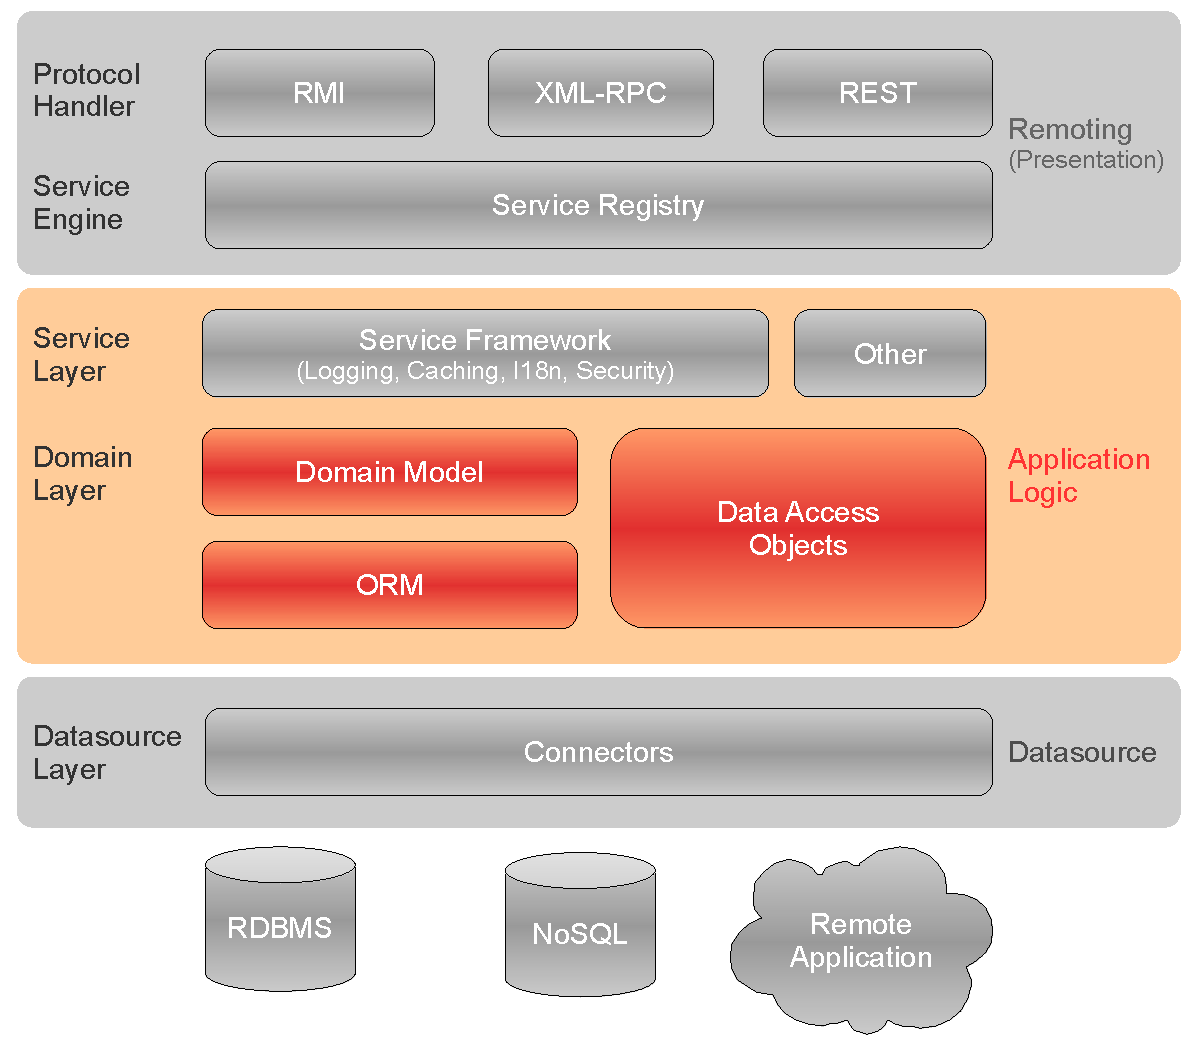
\includegraphics[width=\linewidth]{images/overviews/domain}}
	\caption{Einordnung des Domain Layer}
	\label{ill:domain}
\end{figure}